

\tikzset{every picture/.style={line width=0.75pt}} %set default line width to 0.75pt        

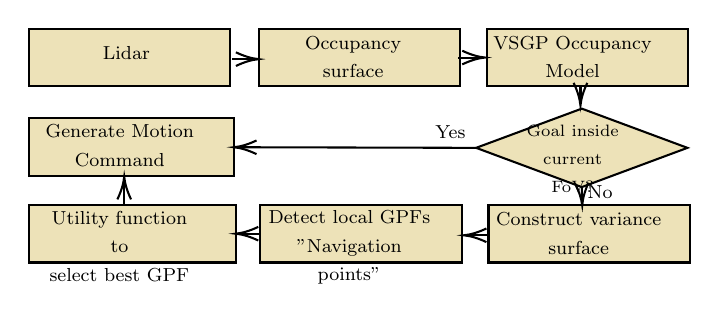
\begin{tikzpicture}[x=0.75pt,y=0.75pt,yscale=-1,xscale=1]
%uncomment if require: \path (0,363); %set diagram left start at 0, and has height of 363

%Shape: Rectangle [id:dp5041996315892758] 
\draw  [fill={rgb, 255:red, 237; green, 226; blue, 184 }  ,fill opacity=1 ] (26,56.11) -- (123.13,56.11) -- (123.13,83.89) -- (26,83.89) -- cycle ;
%Shape: Rectangle [id:dp8950562064101133] 
\draw  [fill={rgb, 255:red, 237; green, 226; blue, 184 }  ,fill opacity=1 ] (246.67,56.11) -- (343.8,56.11) -- (343.8,83.89) -- (246.67,83.89) -- cycle ;
%Shape: Rectangle [id:dp778116150907765] 
\draw  [fill={rgb, 255:red, 237; green, 226; blue, 184 }  ,fill opacity=1 ] (136.76,56.11) -- (233.89,56.11) -- (233.89,83.89) -- (136.76,83.89) -- cycle ;
%Shape: Rectangle [id:dp6736008077761417] 
\draw  [fill={rgb, 255:red, 237; green, 226; blue, 184 }  ,fill opacity=1 ] (26,140.98) -- (125.68,140.98) -- (125.68,168.76) -- (26,168.76) -- cycle ;
%Shape: Rectangle [id:dp7870085085127494] 
\draw  [fill={rgb, 255:red, 237; green, 226; blue, 184 }  ,fill opacity=1 ] (247.52,140.98) -- (344.65,140.98) -- (344.65,168.76) -- (247.52,168.76) -- cycle ;
%Shape: Rectangle [id:dp9576383308440346] 
\draw  [fill={rgb, 255:red, 237; green, 226; blue, 184 }  ,fill opacity=1 ] (137.61,140.98) -- (234.74,140.98) -- (234.74,168.76) -- (137.61,168.76) -- cycle ;
%Flowchart: Decision [id:dp028452627812187714] 
\draw  [color={rgb, 255:red, 0; green, 0; blue, 0 }  ,draw opacity=1 ][fill={rgb, 255:red, 237; green, 226; blue, 184 }  ,fill opacity=1 ] (292.46,94.61) -- (343.37,113.51) -- (292.46,132.42) -- (241.56,113.51) -- cycle ;
%Shape: Rectangle [id:dp5948260780362231] 
\draw  [fill={rgb, 255:red, 237; green, 226; blue, 184 }  ,fill opacity=1 ] (26,99.32) -- (124.83,99.32) -- (124.83,127.1) -- (26,127.1) -- cycle ;
%Straight Lines [id:da8537430744371559] 
\draw    (123.98,70.77) -- (134.76,70.77) ;
\draw [shift={(136.76,70.77)}, rotate = 180] [color={rgb, 255:red, 0; green, 0; blue, 0 }  ][line width=0.75]    (10.93,-3.29) .. controls (6.95,-1.4) and (3.31,-0.3) .. (0,0) .. controls (3.31,0.3) and (6.95,1.4) .. (10.93,3.29)   ;
%Straight Lines [id:da611129628998444] 
\draw    (233.04,70) -- (243.82,70) ;
\draw [shift={(245.82,70)}, rotate = 180] [color={rgb, 255:red, 0; green, 0; blue, 0 }  ][line width=0.75]    (10.93,-3.29) .. controls (6.95,-1.4) and (3.31,-0.3) .. (0,0) .. controls (3.31,0.3) and (6.95,1.4) .. (10.93,3.29)   ;
%Straight Lines [id:da7956834446453471] 
\draw    (246.67,155.64) -- (237.59,155.64) ;
\draw [shift={(235.59,155.64)}, rotate = 360] [color={rgb, 255:red, 0; green, 0; blue, 0 }  ][line width=0.75]    (10.93,-3.29) .. controls (6.95,-1.4) and (3.31,-0.3) .. (0,0) .. controls (3.31,0.3) and (6.95,1.4) .. (10.93,3.29)   ;
%Straight Lines [id:da19366340312569585] 
\draw    (136.76,154.87) -- (127.68,154.87) ;
\draw [shift={(125.68,154.87)}, rotate = 360] [color={rgb, 255:red, 0; green, 0; blue, 0 }  ][line width=0.75]    (10.93,-3.29) .. controls (6.95,-1.4) and (3.31,-0.3) .. (0,0) .. controls (3.31,0.3) and (6.95,1.4) .. (10.93,3.29)   ;
%Straight Lines [id:da8231916649130704] 
\draw    (241.56,113.51) -- (126.83,113.21) ;
\draw [shift={(124.83,113.21)}, rotate = 0.15] [color={rgb, 255:red, 0; green, 0; blue, 0 }  ][line width=0.75]    (10.93,-3.29) .. controls (6.95,-1.4) and (3.31,-0.3) .. (0,0) .. controls (3.31,0.3) and (6.95,1.4) .. (10.93,3.29)   ;
%Straight Lines [id:da7821997600551795] 
\draw    (291.83,83.89) -- (291.83,91.14) ;
\draw [shift={(291.83,93.14)}, rotate = 270] [color={rgb, 255:red, 0; green, 0; blue, 0 }  ][line width=0.75]    (10.93,-3.29) .. controls (6.95,-1.4) and (3.31,-0.3) .. (0,0) .. controls (3.31,0.3) and (6.95,1.4) .. (10.93,3.29)   ;
%Straight Lines [id:da7475077440762967] 
\draw    (292.46,132.42) -- (292.63,139.29) ;
\draw [shift={(292.68,141.29)}, rotate = 268.62] [color={rgb, 255:red, 0; green, 0; blue, 0 }  ][line width=0.75]    (10.93,-3.29) .. controls (6.95,-1.4) and (3.31,-0.3) .. (0,0) .. controls (3.31,0.3) and (6.95,1.4) .. (10.93,3.29)   ;
%Straight Lines [id:da8565253571979397] 
\draw    (72.01,141.29) -- (72.01,129.4) ;
\draw [shift={(72.01,127.4)}, rotate = 90] [color={rgb, 255:red, 0; green, 0; blue, 0 }  ][line width=0.75]    (10.93,-3.29) .. controls (6.95,-1.4) and (3.31,-0.3) .. (0,0) .. controls (3.31,0.3) and (6.95,1.4) .. (10.93,3.29)   ;

% Text Node
\draw (60.46,63.54) node [anchor=north west][inner sep=0.75pt]  [xscale=0.85,yscale=0.85] [align=left] {{\footnotesize Lidar}};
% Text Node
\draw (155.05,58.51) node [anchor=north west][inner sep=0.75pt]  [xscale=0.85,yscale=0.85] [align=left] {\begin{minipage}[lt]{45.81pt}\setlength\topsep{0pt}
\begin{center}
{\footnotesize Occupancy }\\{\footnotesize surface}
\end{center}

\end{minipage}};
% Text Node
\draw (246.72,58.65) node [anchor=north west][inner sep=0.75pt]  [xscale=0.85,yscale=0.85] [align=left] {\begin{minipage}[lt]{70.6pt}\setlength\topsep{0pt}
\begin{center}
{\footnotesize VSGP Occupancy }\\{\footnotesize Model}
\end{center}

\end{minipage}};
% Text Node
\draw (261.91,101.02) node [anchor=north west][inner sep=0.75pt]  [xscale=0.85,yscale=0.85] [align=left] {\begin{minipage}[lt]{43.96pt}\setlength\topsep{0pt}
\begin{center}
{\scriptsize Goal inside}\\{\scriptsize current FoV?}
\end{center}

\end{minipage}};
% Text Node
\draw (248.3,143.67) node [anchor=north west][inner sep=0.75pt]  [xscale=0.85,yscale=0.85] [align=left] {\begin{minipage}[lt]{73.02pt}\setlength\topsep{0pt}
\begin{center}
{\footnotesize Construct variance }\\{\footnotesize surface}
\end{center}

\end{minipage}};
% Text Node
\draw (138.92,142.61) node [anchor=north west][inner sep=0.75pt]  [xscale=0.85,yscale=0.85] [align=left] {\begin{minipage}[lt]{71.11pt}\setlength\topsep{0pt}
\begin{center}
{\footnotesize Detect local GPFs }\\{\footnotesize "Navigation points"}
\end{center}

\end{minipage}};
% Text Node
\draw (31.66,142.95) node [anchor=north west][inner sep=0.75pt]  [xscale=0.85,yscale=0.85] [align=left] {\begin{minipage}[lt]{64.86pt}\setlength\topsep{0pt}
\begin{center}
{\footnotesize Utility function to }\\{\footnotesize select best GPF}
\end{center}

\end{minipage}};
% Text Node
\draw (32.64,101.23) node [anchor=north west][inner sep=0.75pt]  [xscale=0.85,yscale=0.85] [align=left] {\begin{minipage}[lt]{63.51pt}\setlength\topsep{0pt}
\begin{center}
{\footnotesize Generate Motion}\\{\footnotesize  Command}
\end{center}

\end{minipage}};
% Text Node
\draw (220.69,101.61) node [anchor=north west][inner sep=0.75pt]  [xscale=0.85,yscale=0.85] [align=left] {{\footnotesize Yes}};
% Text Node
\draw (293.98,130.41) node [anchor=north west][inner sep=0.75pt]  [xscale=0.85,yscale=0.85] [align=left] {{\footnotesize No}};


\end{tikzpicture}